% 第6章第6节：图滤波（滤波问题与谱响应、基于谱分解的滤波、多项式滤波与局部计算、方法比较与结果检验）。

\section{图滤波}
\label{sec:graph-filtering}

图傅里叶变换只换坐标，不改变函数。本节转向改变函数：规定每个模态保留多少、衰减多少，得到新的顶点函数。先定义滤波的目标，再比较两种实现：一种先求谱基再逐模态缩放，另一种只用拉普拉斯的稀疏乘法。若目标响应在图谱上恰好可以由所用多项式表示，两种实现给出同一个输出；若只是用多项式近似，就需要控制输出误差。

\subsection{滤波问题与谱响应}
\label{sec:graph-spec-filtering-problem}

传感器读数常混有逐点跳动的噪声，而真实的温度场在相邻测点间变化平缓。上一节的分解~\eqref{eq:graph-spec-parseval}说明，逐点跳动主要落在大特征值的模态上。于是“去噪”可以表述为：保留小特征值的模态，压低大特征值的模态。把每个模态保留的比例写成特征值的函数，就得到下面的定义。

\begin{definition}[谱滤波]
\label{def:graph-spec-spectral-filter}
给定图算子$\bm L=\bm U\bm\Lambda\bm U^{\top}$、输入$\bm f$和定义在全部特征值上的实函数$g$，称
\begin{equation}
 \bm y=g(\bm L)\bm f=\bm U\,g(\bm\Lambda)\,\bm U^{\top}\bm f,\qquad
 g(\bm\Lambda)=\operatorname{diag}\bigl(g(\lambda_1),\ldots,g(\lambda_n)\bigr)
 \label{eq:graph-spec-spectral-filter}
\end{equation}
为$\bm f$经\term{谱响应}（spectral response）$g$的\term{图滤波}（graph filtering）输出。按谱坐标写，$\widehat y_k=g(\lambda_k)\widehat f_k$。
\end{definition}

$g(\bm L)$正是第~\ref{sec:ls-matrix-functions}节沿特征方向定义的矩阵函数。几种典型响应各有含义：$g\equiv1$时$\bm y=\bm f$，原样输出；$g(0)=1$保证零模不变，在正权支撑连通时就是保持各点的平均值；$g$随$\lambda$递减到接近零，则高频模态被压低，输出比输入平缓，这样的响应称为低通。这里规定的是要得到什么输出，下面两小节讨论怎样算出它。

\paragraph{定义的合理性}
$\bm U$不唯一，需要确认输出不依赖它的选取。式~\eqref{eq:graph-spec-spectral-filter}对同一特征值的各个模态使用同一个数$g(\lambda)$，所以$g(\bm L)=\sum_\lambda g(\lambda)\bm P_\lambda$，其中$\bm P_\lambda$是到特征空间的正交投影，只由$\bm L$决定（第~\ref{sec:ls-matrix-functions}节）。重编号也不改变结果：$\bm P\bm L\bm P^{\top}$的特征向量是$\bm P\bm u_k$，特征值不变，于是$g(\bm P\bm L\bm P^{\top})=\bm Pg(\bm L)\bm P^{\top}$，对重排后的输入$\bm P\bm f$输出$\bm P\bm y$，即输出随顶点一起重排。

\paragraph{放大界}
滤波可能把函数放大，放大多少由响应的最大幅度控制。由式~\eqref{eq:graph-spec-parseval}，
\begin{equation}
 \begin{gathered}
 \lVert\bm y\rVert_2^2=\sum_kg(\lambda_k)^2\widehat f_k^{\,2}\leq\Bigl(\max_k|g(\lambda_k)|\Bigr)^2\lVert\bm f\rVert_2^2,\\
 \bm y^{\top}\bm L\bm y=\sum_k\lambda_kg(\lambda_k)^2\widehat f_k^{\,2}\leq\Bigl(\max_k|g(\lambda_k)|\Bigr)^2\bm f^{\top}\bm L\bm f .
 \end{gathered}
 \label{eq:graph-spec-filter-bound}
\end{equation}
所以只要在全部特征值上$|g(\lambda_k)|\leq1$，输出的幅值和沿边变化能量都不会超过输入。没有这个条件，就不能断言滤波不增加幅值或能量；例如$g(\lambda)=1+\lambda$会放大高频模态。

\subsection{基于谱分解的滤波}
\label{sec:graph-spec-eigendecomposition-filter}

最直接的实现照搬定义：先求谱基，再在谱坐标中逐个缩放。

\begin{algorithm}[基于谱分解的图滤波]
\label{alg:graph-spec-eigendecomposition-filter}
输入：$n\times n$实对称图算子$\bm L$，顶点函数$\bm f$，谱响应$g$。输出：$\bm y=g(\bm L)\bm f$。
\begin{enumerate}
 \item 求谱分解$\bm L=\bm U\bm\Lambda\bm U^{\top}$（同一个$\bm L$只需做一次）。
 \item 投影：$\widehat{\bm f}=\bm U^{\top}\bm f$。
 \item 逐模态缩放：$\widehat y_k=g(\lambda_k)\widehat f_k$，$k=1,\ldots,n$。
 \item 重构：$\bm y=\bm U\widehat{\bm y}$。
\end{enumerate}
\end{algorithm}

三步合起来是$\bm U g(\bm\Lambda)\bm U^{\top}\bm f$，正确性直接来自定义。开销要分开计：第1步对稠密矩阵通常需要$O(n^3)$次运算，存储$\bm U$需要$O(n^2)$空间；第2、4步各是一次稠密矩阵乘向量，第3步计算$n$个响应值，合计每个输入$O(n^2)$。图算子固定、要处理许多个输入时，第1步的结果可以反复使用，摊到每个输入上的代价随之下降。若为节省开销只求前若干个模态、把其余模态的响应当作零，就改变了目标响应，实际计算的是另一种截断滤波，需要另行说明误差，不能仍称为原响应的精确实现。

\paragraph{三点路径上的低通滤波}
在单位权三点路径上取$\bm f=(3,1,2)^{\top}$与响应$g(\lambda)=1/(1+\lambda)$。上一节已求出谱坐标$\widehat{\bm f}=(2\sqrt3,\tfrac1{\sqrt2},\tfrac{\sqrt6}2)^{\top}$，三个特征值$0,1,3$的响应为$1,\tfrac12,\tfrac14$，所以
\[
 \bm y=2\sqrt3\,\bm u_1+\tfrac12\cdot\tfrac1{\sqrt2}\,\bm u_2+\tfrac14\cdot\tfrac{\sqrt6}2\,\bm u_3
 =\begin{bmatrix}2\\2\\2\end{bmatrix}+\frac14\begin{bmatrix}1\\0\\-1\end{bmatrix}+\frac18\begin{bmatrix}1\\-2\\1\end{bmatrix}
 =\begin{bmatrix}19/8\\7/4\\15/8\end{bmatrix}.
\]
常量成分$(2,2,2)^{\top}$原样保留，所以输出各分量之和仍为$6$；两个变化成分分别缩小为原来的$\tfrac12$和$\tfrac14$。输出的能量为$(\tfrac58)^2+(\tfrac18)^2=\tfrac{13}{32}\approx0.41$，远小于输入的$5$。这个响应恰好对应求解线性方程组：$g(\bm L)=(\bm I+\bm L)^{-1}$，可以直接核对$(\bm I+\bm L)\bm y=\bm f$。

\subsection{多项式滤波与局部计算}
\label{sec:graph-spec-polynomial-filter}

谱分解的代价主要花在求$\bm U$上。若响应是多项式，可以完全绕开特征向量。设$g(\lambda)=\sum_{r=0}^K\alpha_r\lambda^r$，由$\bm L^r=\bm U\bm\Lambda^r\bm U^{\top}$，
\begin{equation}
 g(\bm L)\bm f=\sum_{r=0}^K\alpha_r\bm L^r\bm f ,
 \label{eq:graph-spec-polynomial-filter}
\end{equation}
右端只需要反复用$\bm L$乘向量。按这种方式计算谱滤波称为\term{多项式图滤波}（polynomial graph filtering）。

\begin{algorithm}[多项式图滤波]
\label{alg:graph-spec-polynomial-filter}
输入：以正权边邻接表存储的$\bm L$，顶点函数$\bm f$，系数$\alpha_0,\ldots,\alpha_K$。输出：$\bm y=\sum_r\alpha_r\bm L^r\bm f$。状态：当前幂次向量$\bm v^{(r)}=\bm L^r\bm f$与累加向量$\bm y$。
\begin{enumerate}
 \item 置$\bm v^{(0)}=\bm f$，$\bm y=\alpha_0\bm f$。
 \item 对$r=1,\ldots,K$：从完整的旧向量$\bm v^{(r-1)}$读取，按$(\bm L\bm v)_i=d_iv_i-\sum_jw_{i,j}v_j$把结果写入另一个缓冲区，得到$\bm v^{(r)}$；再令$\bm y\leftarrow\bm y+\alpha_r\bm v^{(r)}$。
\end{enumerate}
\end{algorithm}

第2步必须同步读取旧向量，理由与第~\ref{sec:graph-spec-neighborhood-aggregation}小节相同：就地改写会让后面的顶点读到本轮的新值，算出的就不再是$\bm L\bm v$。按归纳，每轮结束时$\bm v^{(r)}=\bm L^r\bm f$，$\bm y$累加了前$r$项，所以算法输出式~\eqref{eq:graph-spec-polynomial-filter}。

\paragraph{依赖范围}
多项式滤波的输出只依赖附近的顶点。一次乘法中，$(\bm L\bm v)_i$只读取$v_i$与正权邻居的值。归纳可得，$(\bm L^r\bm v)_i$只依赖在正权支撑图中与$i$相距至多$r$步的顶点：第$r$轮读取的邻居值本身只依赖再远$r-1$步以内的顶点。所以$K$次多项式滤波在顶点$i$的输出，只依赖$i$的$K$跳邻域。

这是范围的上界，不是说范围内的每个顶点都一定产生非零贡献。单位权三点路径上，$(\bm L^2-3\bm L)\bm e_1=(2,-3,1)^{\top}-3(1,-1,0)^{\top}=(-1,0,1)^{\top}$：顶点$2$与顶点$1$只隔一条边，但两项贡献恰好相消，输出为零。

\begin{figure}[!htb]
  \centering
  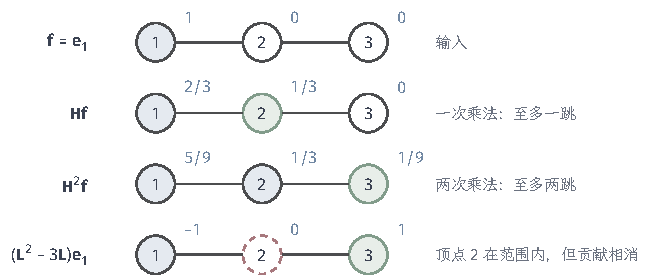
\includegraphics[width=110mm]{figures/01-basic-mathematics/04-graphs/tikz/c6-polynomial-locality/figure.pdf}
  \caption{单位权三点路径上多项式滤波的依赖范围，$\bm H=\bm I-\bm L/3$，蓝色数字为各顶点的输出。从$\bm f=\bm e_1$出发，一次作用只到达一跳邻居（绿色），两次作用才到达两跳外的顶点$3$。最后一行$(\bm L^2-3\bm L)\bm e_1$中，顶点$2$位于范围内，但贡献相消为零（红色虚线）。}
  \label{fig:graph-spec-polynomial-locality}
\end{figure}

图~\ref{fig:graph-spec-polynomial-locality}用一次多项式$\bm H=\bm I-\bm L/3$展示范围怎样扩大。从$\bm e_1$出发，
\[
 \bm H\bm e_1=\bm e_1-\tfrac13(1,-1,0)^{\top}=\bigl(\tfrac23,\tfrac13,0\bigr)^{\top},\qquad
 \bm H^2\bm e_1=\bigl(\tfrac59,\tfrac13,\tfrac19\bigr)^{\top}.
\]
第一轮只有顶点$1$、$2$非零，第二轮才到达顶点$3$。从谱的角度看，$\bm H$的响应$1-\lambda/3$在特征值$0,1,3$上取$1,\tfrac23,0$：常量模态保留，最高频模态被完全消去。

\paragraph{开销与近似误差}
以邻接表存储正权边，一次$\bm L$乘向量要访问每个顶点和每条正权边常数次，需要$O(n+m_+)$次运算；$K$轮共$O(K(n+m_+))$。除了图本身，只需保存旧向量、新向量和累加向量，额外空间为$O(n)$。整个过程不求任何特征向量。

多项式能表示的响应有限，一般的响应$g$只能近似。设多项式$p$在一个包含全部特征值的区间上满足$|g(\lambda)-p(\lambda)|\leq\varepsilon$。对差$g-p$使用放大界~\eqref{eq:graph-spec-filter-bound}，得
\[
 \lVert g(\bm L)\bm f-p(\bm L)\bm f\rVert_2\leq\varepsilon\lVert\bm f\rVert_2 .
\]
所以只要知道谱落在哪个区间，就能把标量函数的逼近误差转成输出误差。对$\bm L_{\mathrm{sym}}$，定理~\ref{thm:graph-spec-normalized-bound}给出区间$[0,2]$；对$\bm L$可用$[0,2d_{\max}]$。图~\ref{fig:graph-spec-filter-responses}(b)在$[0,2]$上逼近低通响应$1/(1+3\lambda)$：用Chebyshev节点插值，$K=2$时最大误差约$0.18$，$K=4$时约$0.038$。

\begin{figure}[!htb]
  \centering
  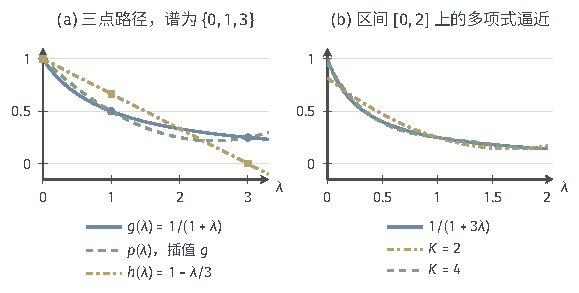
\includegraphics[width=98mm]{figures/01-basic-mathematics/04-graphs/tikz/c6-filter-responses/figure.pdf}
  \caption{谱响应与多项式。(a)~三点路径的谱为$\{0,1,3\}$：蓝色为目标$g(\lambda)=1/(1+\lambda)$，绿色虚线为在三个特征值上与$g$相等的二次多项式$p(\lambda)=1-\tfrac58\lambda+\tfrac18\lambda^2$，二者只在圆点处重合；黄色点划线为$h(\lambda)=1-\lambda/3$，方点是它在特征值上的取值。(b)~区间$[0,2]$上目标$1/(1+3\lambda)$及其$K=2$、$K=4$次Chebyshev节点插值，最大误差约为$0.18$和$0.038$。}
  \label{fig:graph-spec-filter-responses}
\end{figure}

另一种情形是已知全部互不相同的特征值。一个有限集合上的任意函数都可以用插值多项式精确匹配，$s$个不同的特征值需要至多$s-1$次。三点路径的谱为$\{0,1,3\}$，取$p(\lambda)=1-\tfrac58\lambda+\tfrac18\lambda^2$，直接代入得$p(0)=1$、$p(1)=\tfrac12$、$p(3)=\tfrac14$，与$g(\lambda)=1/(1+\lambda)$在三个特征值上相同。于是$p(\bm L)=g(\bm L)$，尽管$p$与$g$作为函数并不相同，见图~\ref{fig:graph-spec-filter-responses}(a)。这种精确匹配要求事先知道特征值，在大图上通常做不到。

\subsection{方法比较与结果检验}
\label{sec:graph-spec-filter-comparison}

比较两种实现时，要固定同一个图算子、同一个输入和同一个目标响应，只比较计算方式。表~\ref{tab:graph-spec-filter-comparison}列出主要差别。

\begin{table}[!htb]
  \centering\small
  \begin{tabularx}{\linewidth}{@{}lXX@{}}
    \toprule
    & 基于谱分解（算法~\ref{alg:graph-spec-eigendecomposition-filter}） & 多项式滤波（算法~\ref{alg:graph-spec-polynomial-filter}）\\
    \midrule
    预处理 & 稠密特征分解，$O(n^3)$ & 无；逼近一般响应时需要谱区间 \\
    单个输入 & $O(n^2)$ & $O(K(n+m_+))$ \\
    额外存储 & $\bm U$，$O(n^2)$ & 三个向量，$O(n)$ \\
    适用响应 & 任意$g$，精确 & 多项式精确；一般$g$有误差$\varepsilon\lVert\bm f\rVert_2$ \\
    \bottomrule
  \end{tabularx}
  \caption{同一图算子、输入和目标响应下两种滤波实现的比较。$n$为顶点数，$m_+$为正权边数，$K$为多项式次数。}
  \label{tab:graph-spec-filter-comparison}
\end{table}

多项式响应可以用两种方法实现同一个算子，结果相同；用多项式逼近一般响应，则在实现方式之外又改变了目标，多出一项近似误差。这两种差别要分开说明，不能把“实现方式不同”和“目标响应不同”混为一谈。

\paragraph{交叉核对}
在小图上，可以用两种实现互相核对。仍取三点路径、$\bm f=(3,1,2)^{\top}$，用插值多项式$p$按算法~\ref{alg:graph-spec-polynomial-filter}计算：$\bm L\bm f=(2,-3,1)^{\top}$，$\bm L^2\bm f=(5,-9,4)^{\top}$，
\[
 p(\bm L)\bm f=\bm f-\tfrac58\bm L\bm f+\tfrac18\bm L^2\bm f
 =\Bigl(3-\tfrac{10}8+\tfrac58,\ 1+\tfrac{15}8-\tfrac98,\ 2-\tfrac58+\tfrac48\Bigr)^{\top}
 =\Bigl(\tfrac{19}8,\tfrac74,\tfrac{15}8\Bigr)^{\top},
\]
与谱分解的结果完全一致，而这次计算没有用到任何特征向量。还可以检查几项必然成立的性质：$\max_k|g(\lambda_k)|=1$，按放大界应有$\lVert\bm y\rVert_2^2\leq\lVert\bm f\rVert_2^2$，实际为$\tfrac{782}{64}\approx12.2\leq14$；$g(0)=1$且图连通，各分量之和应保持为$6$；把顶点重编号后重算，输出应随之重排。

本节的滤波只依赖有限维谱分解，没有引入时间。连续的热扩散及其时间离散会给出特定的响应族，它们在后续过程与信号部分建立。
